% main.tex -- draft for IEEE QCE 2027 (full paper, ~8 pp. + refs)
% Compile: latexmk -pdf main.tex
%
% TITLE OPTIONS (pick one):
%  (1) Where Error Mitigation Stops Paying: Equal-Budget Twirled CDR, Matched-Cost ZNE
%      Controls, and Identity Insertion on a Five-Qubit Star Processor
%  (2) Paying for Mitigation: A Budget-Controlled Hardware Study of ZNE, CDR and Pauli
%      Twirling under Routing Overhead
%  (3) Fair Comparisons of Quantum Error Mitigation under Routing Overhead on a
%      Star-Topology Superconducting Processor
%
% STATUS: window w01, nights A and P5 analysed; night B (30 and 57 CZ) pending.
% Every \TBD{...} is a placeholder for night-B numbers or for items still to be supplied.
% All other numbers are computed from runs/odra_campaign/w01{A,P5}/*.csv,
% results/depth_regression_w01P5.csv and runs/odra_pilot/* (pilot, exploratory).

\documentclass[conference]{IEEEtran}
\IEEEoverridecommandlockouts
\usepackage[T1]{fontenc}
\usepackage[utf8]{inputenc}
\usepackage{amsmath,amssymb,mathtools}
\usepackage{booktabs}
\usepackage{graphicx}
\usepackage{xcolor}
\usepackage{url}
\usepackage[hidelinks]{hyperref}
\usepackage{cite}

\newcommand{\TBD}[1]{\textcolor{red}{\textbf{[TBD: #1]}}}
\newcommand{\ev}[1]{\langle #1\rangle}
\newcommand{\ket}[1]{|#1\rangle}
\newcommand{\Oid}{O_{\mathrm{id}}}
\newcommand{\CZ}{\mathrm{CZ}}
\newcommand{\PRX}{\mathrm{PRX}}
\newcommand{\Var}{\operatorname{Var}}
\newcommand{\Cov}{\operatorname{cov}}
\newcommand{\E}{\mathbb{E}}
\newcommand{\arm}[1]{\texttt{#1}}

\begin{document}

\title{Where Error Mitigation Stops Paying: Equal-Budget Twirled CDR, Matched-Cost ZNE
Controls, and Identity Insertion on a Five-Qubit Star Processor}

\author{\IEEEauthorblockN{Karina Le\'skiewicz}
\IEEEauthorblockA{KN Axion, Wroc{\l}aw University of Science and Technology
(Politechnika Wroc{\l}awska), Poland}}

\maketitle

% ---------------------------------------------------------------------------------------
\begin{abstract}
Quantum error mitigation (QEM) methods are usually compared at whatever shot budget each
happens to use, which conflates bias removal with plain averaging and hides where a method
stops paying for its overhead. We compare zero-noise extrapolation (ZNE), Clifford data
regression (CDR) and CDR with Pauli twirling on the five-qubit star-topology IQM ODRA~5
processor, using one frozen variational classifier compiled along a routing ladder of
12, 30, 39 and 57 CZ gates. All CDR arms spend an identical budget of 1,032,192 shots per
evaluation point; ZNE is accompanied by matched-cost garbage- and identity-folding controls.
In the first calibration window (12 and 39 CZ, 8 points each), native Pauli twirling lowers
the CDR error at 39 CZ from 0.053 to 0.040 (7/8 pairs, geometric-mean ratio 0.68) and has no
effect at 12 CZ, where the error is already near the shot-noise level. ZNE beats garbage
folding at 12 CZ (0.045 vs.\ 0.137), but at 39 CZ its apparent gain over raw estimation is
matched by garbage folding (0.112 vs.\ 0.103): Richardson extrapolation has degenerated into a
rescaled single measurement, which neither negative-mass nor SNR diagnostics flagged. An
identity-insertion experiment shows that raw error is driven by circuit duration
($\times1.43$ per~\textmu s, $p<10^{-4}$) rather than CZ count at fixed duration, while after
CDR the CZ-driven part remains ($\times1.34$ per 10 CZ, $p=0.002$). The 30- and 57-CZ rungs
and the pre-registered confirmatory tests are pending: \TBD{night-B result for H1/H3/H6 in one
sentence}.
\end{abstract}

\begin{IEEEkeywords}
quantum error mitigation, zero-noise extrapolation, Clifford data regression, Pauli
twirling, superconducting qubits, routing overhead, pre-registration
\end{IEEEkeywords}

% ---------------------------------------------------------------------------------------
\section{Introduction}

A quantum processor does not return an expectation value $\ev{O}$; it returns bitstrings,
from which $\ev{O}$ is estimated. Quantum error mitigation (QEM) replaces a single
estimate by a classical post-processing of many, possibly modified, circuit executions,
so that the bias introduced by hardware noise is reduced at the price of a larger
variance~\cite{temme2017,li2017,cai2023}. The price is not small. Lower bounds on the
sampling overhead of any QEM method grow exponentially with the amount of noise in the
circuit~\cite{takagi2022,quek2024}. For every method, therefore, a circuit size exists beyond
which the shots spent on mitigation buy less accuracy than the same shots spent on plain
estimation, or beyond which the method stops working at all. Locating that boundary on
real hardware, for realistic workloads, is a practical question for anyone running
near-term algorithms.

Two features of current comparisons make the boundary hard to see. First, methods are often
compared at unequal budgets. A Pauli-twirled estimator averages over $M$ random frames; if
its untwirled baseline is measured once, part of any improvement is just $M$-fold
averaging. Second, two-qubit gate counts on hardware are not set by the algorithm alone:
on a sparsely connected device, routing inserts SWAP gates whose CZs carry most of the
noise. The same logical circuit can cost very different numbers of CZ gates on different
topologies, so a statement such as ``method X works up to depth $d$'' is ill-posed unless the
compiled gate count is controlled.

In this work we use a single frozen workload---a five-qubit data-re-uploading classifier
compiled for a star-coupled processor---to build a controlled ladder of compiled CZ counts
(12, 30, 39, 57), and we measure on hardware where ZNE, CDR and Pauli twirling pay off along
it. Our contributions are:
\begin{itemize}
  \item \textbf{An equal-budget design for learning-based mitigation.} Every CDR arm spends
  exactly $(n_{\text{train}}+1)MS$ shots per point; an \arm{off\_copies} control averages $M$
  identical copies, so the difference to a twirled arm isolates twirling from averaging.
  Single-qubit merging after native twirling keeps the twirled circuits at the gate count
  of the untwirled ones.
  \item \textbf{A hardware observation of ZNE degeneracy under signal collapse.} At 39~CZ,
  ZNE's gain over raw estimation is reproduced by a matched-cost garbage-folding control, and
  a floor-tracking distance of 0.016 confirms that the extrapolation is a rescaled first
  measurement. Negative-mass and SNR diagnostics did not detect it; garbage folding did.
  We also report that an identity-folding control, valid in simulation, is invalid on
  hardware.
  \item \textbf{A decomposition of what drives the error.} Identity insertion (CZ$\cdot$CZ
  pairs vs.\ duration-matched idling) on the fixed 12-CZ circuit separates CZ count from
  duration: raw error follows duration, while the residual after CDR follows CZ count.
  \item \textbf{A pre-registered analysis plan}, frozen with its code before any analysis of
  the window, with its status reported honestly (pre-analysis, not pre-data), and pilot
  measurements of the ZNE variance constant $\kappa$ and of classifier decision changes,
  labelled as exploratory.
\end{itemize}

Section~\ref{sec:background} gives the noise model and the three methods; Section~\ref{sec:methods}
the device, workload and design; Section~\ref{sec:results} the results; Section~\ref{sec:discussion}
discusses them together with the limitations of a single-device, single-window study.

% ---------------------------------------------------------------------------------------
\section{Background}\label{sec:background}

\subsection{Noise as signal compression}
A noisy device implements a channel $\tilde{\mathcal C}$ instead of the unitary $U_C$, so we
estimate $E=\mathrm{Tr}[O\tilde{\mathcal C}(\rho_0)]$ rather than
$\Oid=\mathrm{Tr}[O\,U_C\rho_0U_C^\dagger]$. A mitigation method chooses circuits
$C_1,\dots,C_K$, measures their $E_k$ and returns $\hat O=g(E_1,\dots,E_K)$; the quantum state
itself stays noisy. Its quality is the mean squared error
$\mathrm{MSE}=B^2+\Var\hat O$ with bias $B=\E\hat O-\Oid$.

The model behind both methods studied here is global depolarization. A depolarizing channel
$\mathcal D_p(\rho)=(1-p)\rho+pI/2^n$ commutes with every unitary, so $N$ such channels spread
through a circuit can be collected at its end. If noise is amplified $\lambda$-fold and
$\gamma=pN$,
\begin{equation}
  E(\lambda)\approx f+(\Oid-f)\,e^{-\gamma\lambda},
  \label{eq:compress}
\end{equation}
where $f$ is the \emph{floor}, the value of $\ev{O}$ under full decoherence. For the mean-$Z$
observable used here, $f=0$ under pure depolarization, but $T_1$ relaxation pulls qubits
towards $\ket0$, i.e.\ $Z=+1$, so on transmons $f>0$ and must be measured. The raw bias is
$B\approx-\gamma(\Oid-f)$, and recovering $\Oid$ divides the shot noise by $e^{-\gamma}$ as
well, which is the origin of the exponential sampling cost~\cite{takagi2022,quek2024}.
Equation~\eqref{eq:compress} is exact only for global depolarization; local, correlated and
coherent noise break it, and that is where both methods' boundaries come from.

\subsection{Zero-noise extrapolation, the constant $\kappa$, and degeneracy}
ZNE~\cite{temme2017,li2017,kandala2019} amplifies noise and extrapolates back. With global
folding~\cite{giurgica2020}, $U\to U(U^\dagger U)^k$ leaves the function unchanged but
multiplies the gate count by $\lambda=2k+1$; we use $\lambda\in\{1,3,5\}$. Richardson
extrapolation evaluates the Lagrange polynomial through $(\lambda_k,E_k)$ at zero,
$\hat E(0)=\sum_k c_kE(\lambda_k)$ with $c_k=\prod_{j\neq k}\lambda_j/(\lambda_j-\lambda_k)$; for
$\{1,3,5\}$, $c=(\tfrac{15}{8},-\tfrac54,\tfrac38)$ and $\sum_kc_k=1$, so a constant floor passes
through unchanged. The interpolation remainder gives $|B_{\text{ZNE}}|\lesssim
2.5\,\gamma^3|\Oid-f|$, i.e.\ bias of order $\gamma^3$ instead of $\gamma$ for small $\gamma$.

\emph{Lower edge.} The coefficients are large and of alternating sign, so shot noise is
amplified. Splitting $S$ shots equally over $|\Lambda|$ scales,
\begin{equation}
  \mathrm{MSE}_{\text{ZNE}}-\mathrm{MSE}_{\text{raw}}=\kappa\frac{V}{S}+\bigl(B_{\text{ZNE}}^2-B^2\bigr),
  \label{eq:kappa}
\end{equation}
with $\kappa=|\Lambda|\sum_kc_k^2-1$ and $V$ the single-shot variance. ZNE helps only above $S^\ast=\kappa V/(B^2-B_{\text{ZNE}}^2)$
\cite{krebsbach2022,scavino2026}. $\kappa$ depends only on the nodes and the allocation:
$4.00$, $14.66$ and $44.56$ for $\{1,3\}$, $\{1,3,5\}$, $\{1,3,5,7\}$. A Neyman allocation
$n_k\propto|c_k|\sigma_k$ minimizes the variance and gives
$\kappa_{\text{opt}}=(\sum_k|c_k|\sigma_k/\sigma_1)^2-1$ ($3.0$, $11.25$, $35.0$ for equal
$\sigma_k$). Because $\kappa$ does not depend on the circuit, it is a falsifiable prediction.

\emph{Upper edge.} When the circuit is deep enough that $E(3)\approx E(5)\approx f$, then
$\hat E(0)=c_1E_1+(1-c_1)f=\tfrac{15}{8}E_1-\tfrac78f$: the ``extrapolation'' is a rescaling of a
single measurement, which can look like successful mitigation when the compression at
$\lambda=1$ happens to be about $8/15$. K\"oster and Mauerer reported this degeneracy on a
54-qubit IQM device~\cite{koster2026}. It is invisible in the scalar $\hat E$, so we use three
diagnostics: (i) a \emph{garbage-folding} control $U(V^\dagger U)^k$, where $V$ has the same CZ
skeleton and PRX count as $U$ but random angles---same cost, function destroyed, so any
``gain'' it reproduces is an artefact; (ii) the negative mass $W_{\text{neg}}=\sum_s\max(0,
-\sum_kc_kP_s(\lambda_k))$ of Richardson applied to each of the $2^5$ outcome probabilities;
(iii) $\mathrm{SNR}=|E(\lambda_{\max})|/\mathrm{SE}$. We also report the floor-tracking distance
$|\hat E-(c_1E_1+(1-c_1)f)|$, small when $\hat E$ is just a rescaled $E_1$.

\subsection{Clifford data regression and errors in variables}
CDR~\cite{czarnik2021,lowe2021,bultrini2023} replaces the rotation angles of the target circuit
by Clifford values, measures these training circuits on the device, computes their ideal
values efficiently with a stabilizer simulator~\cite{gottesman1998,aaronson2004}, and fits
$\Oid\approx aE+b$, which it then applies to the measured target. Under depolarization
$E=(1-p)\Oid+pf$ is affine in $\Oid$ with the same coefficients for every circuit sharing the
noise, so a line learned on Cliffords transfers; affine readout error is corrected along
the way. Two effects break the transfer. Coherent errors act through interference that
depends on the specific circuit, scattering training points about the line and lowering
$r^2$. And the regressors $x_i$ are themselves shot-noise estimates, which attenuates the OLS
slope by $\Var x^\star/(\Var x^\star+\bar\sigma_x^2)$ (regression dilution). The
errors-in-variables (EIV) estimator $a_{\text{EIV}}=\Cov(x,y)/(\Var x-\bar\sigma_x^2)$
\cite{fuller1987} removes the attenuation but becomes unstable when the true spread of $x$ is
small; we cap its de-attenuation at $4\times$ and report OLS as primary.

\subsection{Pauli twirling}
For a Pauli $A$ and the Clifford CZ, $B=\CZ\,A\,\CZ^\dagger$ is a Pauli and $B\,\CZ\,A=\CZ$,
so wrapping each CZ in a random frame $(A,B)$ leaves the circuit's function unchanged
\cite{wallman2016,hashim2021}. Writing the gate error in its process ($\chi$-matrix) form,
$\Lambda(\rho)=\sum_{\alpha\beta}\chi_{\alpha\beta}P_\alpha\rho P_\beta$, and averaging over the
two-qubit Paulis, the signs $(-1)^{\langle k,\alpha\rangle+\langle k,\beta\rangle}$ average to
$\delta_{\alpha\beta}$, so
\begin{equation}
  \Lambda_{\text{tw}}(\rho)=\sum_\alpha\chi_{\alpha\alpha}P_\alpha\rho P_\alpha .
\end{equation}
Twirling preserves the diagonal (the Pauli error rates, hence the process fidelity) and
removes the off-diagonal, coherent part. For example, a coherent $ZZ$ rotation by $\theta$
repeated $N$ times gives an infidelity $\approx N^2\theta^2/4$, and $\approx N\theta^2/4$ after
twirling. This motivates twirling as a precondition for CDR, whose single affine map is
better matched by a Pauli channel than by a circuit-dependent coherent error. In practice
only $M$ frames are sampled ($M=6$ here), each a separate circuit, which multiplies the
measurement cost by $M$ and is why an equal-budget comparison is needed. We stress that the
argument above is a motivation, not an explanation of our data: twirling helps empirically,
but the mechanism goes beyond a simple coherent $ZZ$ error on the CZ (Section~\ref{sec:discussion}).

% ---------------------------------------------------------------------------------------
\section{Methods}\label{sec:methods}

\subsection{Device and compilation}
All new data come from IQM ODRA~5, a five-transmon processor with star coupling (hub QB3).
Native gates are $\PRX(\theta,\varphi)=e^{-i\frac\theta2(\cos\varphi X+\sin\varphi Y)}$ and CZ,
the latter only on hub edges; $Z$ rotations are virtual. In a device calibration dump of
2026-08-03, interleaved randomized benchmarking gave CZ errors of 0.78--1.05\% on the four hub
edges and PRX errors of 0.10--0.12\%, so the CZ count is the natural cost axis.

There is a single compilation path: Qiskit~\cite{qiskit2024} 2.4.1 \texttt{transpile} to
$\{\texttt{r},\texttt{cz}\}$ on the star coupling map with the identity layout (logical qubit 0 on
the hub), optimization level 1 and a fixed \texttt{seed\_transpiler}=42, followed by our own
single-qubit merging pass. We found that an unseeded path was non-deterministic: five
compilations of one routed circuit gave five distinct CZ skeletons, and CDR training circuits
compiled separately matched their target's routing in only 0--2 of 10 cases, which invalidates
the premise that training and target circuits see the same noise. With the fixed path the
compilation is bit-reproducible and training circuits are built on the target's
\emph{native} circuit, so they share its CZ skeleton by construction.

\emph{Single-qubit merging.} Every run of single-qubit gates between two CZs on a wire is fused
into at most one PRX: any $SU(2)$ element is $R_Z(\alpha)\PRX(\theta,\varphi)$ up to phase;
$R_Z$ commutes with CZ (both diagonal) and is pushed into the next run as a phase shift; a
trailing $R_Z$ before $Z$-basis readout is dropped. The CZ skeleton is never modified, and the
code checks that no wire carries two consecutive single-qubit gates. Merging matters for
twirling: emitted as separate pulses, the Pauli frames lengthen the circuit (on the 12-CZ
circuit, from 40 to 92 single-qubit gates before merging), and an earlier native-twirling run
without merging came back negative for that reason. With merging, applied to \emph{all} arms,
the target circuits carry 20 PRX (untwirled) and 23--27 PRX (twirled) at 12~CZ, and 80 and
80--83 PRX at 39~CZ.

\subsection{Workload and routing ladder}
The workload is a binary classifier on the \emph{two curves} dataset of
\texttt{qml\_benchmarks}~\cite{bowles2024} (300 samples, 8 features, degree-8 curves offset by
0.1, Gaussian noise 0.01; features scaled to $[-\pi,\pi]$; stratified 180/120 split, seed 42).
The model is a hardware-efficient ansatz~\cite{kandala2017} with data re-uploading
\cite{perezsalinas2020,schuld2021}: $n=5$ qubits, $L=3$ layers, each layer applying
$R_X(w^{\text{enc}}_{\ell q}x_{(5\ell+q)\bmod 8})$, trainable $R_YR_Z$ rotations and a CX
entangling block, followed by a final $R_YR_Z$ layer; 55 weights in total. The output is
$f(x)=\ev{\bar Z}$, $\bar Z=\frac15\sum_qZ_q$, and the decision is its sign; the margin of a point
is $|\Oid|$.

Four entangling patterns---star, linear, circular, all-to-all (12, 12, 15 and 30 logical
two-qubit gates)---are each trained separately (noiseless, MSE loss, Adam with learning rate
0.08, 60 epochs, parameter-shift gradients, seed 42) and frozen; noiseless test accuracies are
0.725, 0.692, 0.675 and 0.767. These are four genuine classifiers of identical capacity rather
than one weight vector transplanted to four topologies. Compiled onto the star, they cost
\textbf{12, 30, 39 and 57 CZ}: every non-star gate must be routed through the hub, and each SWAP
adds three CZ. This routing ladder is the cost axis of the study.

\subsection{CDR arms at equal budget}
Every CDR arm uses $n_{\text{train}}=20$ training circuits (including a nearest-Clifford
anchor), $M=6$ and $S=8192$, and spends
\begin{equation}
  B_{\text{CDR}}=(n_{\text{train}}+1)\,M\,S=1{,}032{,}192
\end{equation}
shots per evaluation point.
The target is always measured $M$ times; the arms differ only in how the training half is
spent (Table~\ref{tab:arms}). Because the mean of $M$ measurements of $S$ shots has variance
$V/(MS)$ whether they are copies or frames, \arm{twirl\_native} vs.\ \arm{off\_copies}
isolates twirling from averaging (frames add frame-to-frame variance, so the comparison if
anything disfavours twirling). In \emph{logical} twirling the frames wrap the logical
entangling gates before routing, so SWAP-derived CZs stay bare (only 40\%, 38\% and 53\% of CZs
are wrapped at 30, 39 and 57~CZ); \emph{native} twirling wraps every physical CZ after routing
and is followed by merging. Training angles are drawn by a \arm{near\_target} sampler
(Clifford angles weighted by $e^{-d^2/\sigma^2}$, $d$ the angular distance to the target angle,
$\sigma=\pi/4$) seeded per (base seed, point, window), so each point has its own training set;
the logical-vs-native comparison uses a common \arm{shared\_random} set so that only the
placement of frames differs.

\begin{table}[t]
\caption{CDR arms; all spend $(n_{\text{train}}+1)MS$ shots per point.}
\label{tab:arms}
\centering\footnotesize
\begin{tabular}{@{}lll@{}}
\toprule
arm & training circuits $\times$ repeats & role \\
\midrule
\arm{off\_copies} & $n_{\text{train}}\times M$ identical copies & control \\
\arm{twirl\_native} & $n_{\text{train}}\times M$ frames, after routing, merged & main test \\
\arm{twirl\_logical} & $n_{\text{train}}\times M$ frames, before routing & variant \\
\arm{spread} & $n_{\text{train}}M$ distinct circuits $\times$ 1 frame & proposal \\
\bottomrule
\end{tabular}
\end{table}

\arm{spread} spends the same budget on $n_{\text{train}}M=120$ distinct near-target circuits with
one frame each. Its motivation is fit degeneracy: deep Clifford circuits scramble stabilizers,
so $\ev{\bar Z}=0$ for most training circuits; if a fraction $q\approx0.2$ is informative, a
20-point fit rests on at most one informative point with probability $\approx0.07$, a 120-point
fit almost never. Its price is that each point is measured once, so regression dilution is
stronger and the EIV variance must be modelled (shot model plus the frame-to-frame variance
measured on the target).

\subsection{ZNE with matched-cost controls}
ZNE uses global folding at $\lambda\in\{1,3,5\}$ on the already-compiled native circuit, never
re-transpiled (re-transpiling would let the optimizer cancel $U^\dagger U$), with barriers
between folds, $S=8192$ shots per scale (24,576 per point) and Richardson extrapolation
without clamping: estimates outside $[-1,1]$ are flagged as unphysical, not replaced. Three
variants share the $\lambda=1$ measurement and have identical CZ skeletons and PRX counts at
every scale: \emph{genuine} folding; \emph{garbage} folding with a random-angle twin $V$ (one
$V$ per point, seeded); and \emph{identity} folding, a block with the CZ sequence of
$U^\dagger U$ in which each single-qubit gate is paired with its inverse so that the CZs
multiply to the identity. The floor $f$ is taken as the garbage-folding value at
$\lambda=5$. Pre-registered thresholds: median $W_{\text{neg}}\le0.02$ (from a depolarizing
null at 8192 shots, 99th percentile 0.014) and median SNR at $\lambda=5$ $\ge2$.

\subsection{Identity insertion (P5)}
A deeper circuit changes CZ count, PRX count and duration at once. To separate them we keep
the star classifier fixed (12~CZ) and insert $k\in\{6,12,20\}$ identity pairs at evenly spread
CZ positions: \emph{cz\_pairs} inserts $\CZ\cdot\CZ=I$ on the edge of an existing CZ (24, 36,
52~CZ; same PRX and function, $2k$ CZ durations longer), and \emph{idle\_matched} inserts a
delay of two CZ durations on both qubits at the same positions (12~CZ, same duration as
cz\_pairs). Pairs are fenced by barriers. Insertion positions depend only on the CZ index, so
targets and their training circuits receive identical insertions and CDR's skeleton match
survives. The star classifiers with $L=6,9,13$ layers (24, 36, 52~CZ) add PRX on top but are
different models, so the primary analysis uses the $L=3$ rungs only. Durations are ASAP
schedule lengths (parallel gates counted once, waiting included; $t_{\text{CZ}}=60$\,ns,
$t_{\text{PRX}}=20$\,ns), ranging from 0.80\,\textmu s (base) to 3.20\,\textmu s (52 CZ or
matched idle) and 3.40\,\textmu s ($L=13$). We fit
\begin{equation}
  \log\varepsilon_{ij}=\alpha_i+\beta_{\text{CZ}}\,\tfrac{n_{\text{CZ},j}}{10}+\beta_t\,t_j[\text{\textmu s}]+u_{ij}
\end{equation}
with point fixed effects $\alpha_i$ and standard errors clustered by point; $e^\beta$ is the
multiplicative change of the error per 10 CZ or per microsecond. Only the
\arm{off\_copies} arm is run in this night, without ZNE.

\subsection{Evaluation points, window and nights}
From the 100 frozen reference points of the test set we select 24, stratified by the star
model's ideal margin $|\Oid|$ (four quartiles, six points evenly spaced in rank within each);
the selection is deterministic and committed. A window uses 8 of them (point set 0: two per
quartile). The primary metric is the per-point absolute error
$\varepsilon=|\hat O-\Oid|$; accuracy is secondary because with 8 points it is extremely noisy.

Window \texttt{w01} consists of three nights (Table~\ref{tab:nights}). All arms of a rung run
in the same night and calibration; a shallow and a deep rung are paired per night. Within a
night, a block is one (rung, arm) or (rung, ZNE) unit, and the block order is randomized with
the window seed and recorded in the manifest. The device's calibration-set identifier is read
before and after every block; a block in which it changes, or in which it differs from the
first block of the night, is flagged. Night A ran on a single calibration set
(10,192 circuits; the run was interrupted once and resumed with identical seeds, records
spanning 08:20--20:39 UTC on 2026-10-24). In night P5 (10,080 circuits, 2026-10-24/25) the
calibration set changed during the \texttt{star\_cz52} block, and the two subsequent blocks
(\texttt{star\_L6}, \texttt{star\_cz24}) ran on the new set.

\begin{table}[t]
\caption{Nights of window \texttt{w01} (8 evaluation points each).}
\label{tab:nights}
\centering\footnotesize
\begin{tabular}{@{}lll@{}}
\toprule
night & rungs (CZ) & content \\[-1pt]
\midrule
A  & star 12, circular 39 & 5 CDR arms; ZNE, 3 variants \\
B  & linear 30, all-to-all 57 & as A; \TBD{status} \\
P5 & star 12; +6/12/20 CZ pairs; & \arm{off\_copies} only \\
   & +matched idle; $L$=6/9/13 & (no ZNE) \\
\bottomrule
\end{tabular}
\end{table}

\subsection{Statistics and pre-registration}
Comparisons are paired on (rung, point), on $\log\varepsilon$ (effects are multiplicative and
errors skewed; zero errors are floored at $10^{-4}$), with one-sided Wilcoxon signed-rank tests
\cite{wilcoxon1945} and geometric-mean ratios with percentile bootstrap CIs. The primary family
is H1 (twirling lowers CDR error at equal budget, \arm{twirl\_native} vs.\ \arm{off\_copies},
32 pairs over nights A+B), H3 (native at least as good as logical), H6 (\arm{spread} beats
\arm{twirl\_native}), H7a (more CZ at fixed duration raises raw error) and H7b (longer duration
at fixed gates raises raw error), with Holm correction~\cite{holm1979} at $\alpha=0.05$.
Secondary: H4, the ZNE window per rung (ZNE below raw, one-sided Wilcoxon over 8 points,
$p<0.05$; below garbage; median $W_{\text{neg}}\le0.02$; median SNR $\ge2$), and H5, decision
agreement with the ideal classifier (exact McNemar test~\cite{mcnemar1947}), where the claim
tested is that decision changes occur below the median margin.

The plan (\texttt{preregistration.md}) and the code that executes it
(\texttt{analysis/prereg\_w01.py}) were committed and tagged \texttt{prereg-v1} before any error,
ratio, fit or test of \texttt{w01} was computed~\cite{nosek2018}. \emph{Honest status:} this is a
pre-analysis plan, not a pre-data registration---night A was already collecting raw counts when
the plan was written. Pilot windows (2026-10-23/24) were analysed and informed the hypotheses;
they are exploratory and enter no confirmatory test. One inconsistency was found while
drafting: the plan text describes H7 as two-sided while the frozen code tests it one-sided in
the registered direction; we report both and neither changes the outcome.

\subsection{Reproducibility}
Every circuit has a deterministic identifier and seed (frames, garbage twins, training sets).
Raw counts of every circuit are archived (\texttt{counts.jsonl}) together with a manifest holding
the git commit, block order, job identifiers and calibration-set IDs; for twirled circuits the
frame (one two-qubit Pauli label per CZ) is stored, which with the native circuit reproduces
the executed circuit exactly. The tables \texttt{cdr.csv} and \texttt{zne.csv} are derived from the
counts alone. The manifests of both nights record the pre-registration commit with a
non-clean working tree; \TBD{state which uncommitted files were present}.

% ---------------------------------------------------------------------------------------
\section{Results}\label{sec:results}

Data status: nights A and P5 of \texttt{w01} are complete. Night B (30 and 57 CZ) is
\TBD{pending / complete}, so H1, H3 and H6 are not yet tested on their pre-registered 32 pairs;
numbers from night A below are descriptive. Table~\ref{tab:main} summarizes the night-A errors.

\begin{table*}[t]
\caption{Mean per-point error $\varepsilon$ over 8 evaluation points (night A, OLS fit), and shots
per evaluation point. Raw: target measured with $M\cdot S=49{,}152$ shots (from the
\arm{off\_copies} arm); in the ZNE comparison the raw reference is the single $\lambda=1$
measurement (8,192 shots): 0.069 and 0.158.}
\label{tab:main}
\centering\footnotesize
\begin{tabular}{@{}rcccccccc@{}}
\toprule
 & & \multicolumn{3}{c}{ZNE $\{1,3,5\}$ folding} & \multicolumn{4}{c}{CDR (equal budget)} \\
\cmidrule(lr){3-5}\cmidrule(l){6-9}
CZ & raw & genuine & garbage & identity & \arm{off\_copies} & \arm{twirl\_native} & \arm{twirl\_logical}$^\dagger$ & \arm{spread} \\
\midrule
12 & 0.074 & 0.045 & 0.137 & 0.072 & 0.022 & 0.015 & 0.019 & 0.012 \\
30 & \TBD{} & \TBD{} & \TBD{} & \TBD{} & \TBD{} & \TBD{} & \TBD{} & \TBD{} \\
39 & 0.161 & 0.112 & 0.103 & 0.194 & 0.053 & 0.040 & 0.025 & 0.068 \\
57 & \TBD{} & \TBD{} & \TBD{} & \TBD{} & \TBD{} & \TBD{} & \TBD{} & \TBD{} \\
\midrule
shots/point & 8,192--49,152 & 24,576 & 24,576 & 24,576 & 1,032,192 & 1,032,192 & 1,032,192 & 1,032,192 \\
\bottomrule
\multicolumn{9}{l}{$^\dagger$ on the \arm{shared\_random} training set; the matching
\arm{twirl\_native} values on that set are 0.031 (12 CZ) and 0.032 (39 CZ).}
\end{tabular}
\end{table*}

\subsection{Twirling at equal budget}
At 39~CZ, native twirling lowered the CDR error from 0.053 to 0.040 at an identical budget, in
7 of 8 pairs (geometric-mean ratio 0.68; sign test $p=0.035$, one-sided Wilcoxon $p=0.074$),
Fig.~\ref{fig:twirl}. At 12~CZ there is no effect: the mean error drops from 0.022 to 0.015, but
only 4 of 8 pairs improve and the geometric-mean ratio is 1.41, driven by two points at which
\arm{off\_copies} happened to land very close to the ideal value ($6\times10^{-4}$ and
$5.5\times10^{-5}$). This is expected: at 12~CZ the CDR error is already of the order of the
statistical error of the fit, and twirling removes a systematic component. Pooled over the
16 night-A pairs, twirling wins 11 (Wilcoxon $p=0.35$, ratio 0.98). The pre-registered H1 on
32 pairs is \TBD{H1: n pairs, Holm-adjusted p, ratio [95\% CI], per-rung ratios at 30 and 57
CZ}. Twirling also raised the median CDR $r^2$ at 39~CZ from 0.83 to 0.92.

On the common training set, logical twirling gave 0.019 / 0.025 and native 0.031 / 0.032
(12 / 39 CZ); native won 7 of 16 pairs. There is no evidence yet for an advantage of native
over logical twirling (H3: \TBD{H3 result on 32 pairs}), even though logical twirling leaves
the SWAP-derived CZs unwrapped.

\emph{Pilot (exploratory).} Three pilot windows on the earlier runner ($n_{\text{train}}=10$,
$M=6$, four evaluation points per rung, rungs 12/57 or 30/39~CZ) gave a lower CDR error with
twirling in 11 of 12 equal-budget pairs: 6/6 for logical twirling (geometric-mean ratio 0.51)
and 5/6 for native twirling (ratio 0.54). The w01 result at 39~CZ is consistent with these; the
absence of a gain at 12~CZ in w01 suggests the pilot's halving was driven by the deeper rungs.

\begin{figure}[t]
\centering
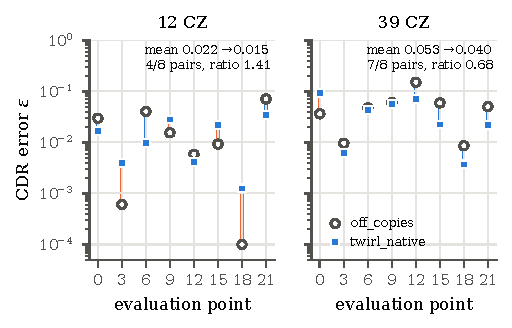
\includegraphics[width=\columnwidth]{figs/fig_twirl_pairs.pdf}
\caption{Per-point CDR error (OLS) of \arm{off\_copies} (circles) and \arm{twirl\_native}
(squares) at equal budget, night A. Blue connectors: twirling better; orange: worse. Ratio:
geometric mean of twirl/off over the 8 points. Errors below $10^{-4}$ are drawn at the
$10^{-4}$ floor used in the analysis (point 18 at 12~CZ: $5.5\times10^{-5}$).}
\label{fig:twirl}
\end{figure}

\subsection{The ZNE window and its degeneracy}
At 12~CZ, ZNE is genuine: it is clearly better than garbage folding (0.045 vs.\ 0.137, 7/8
pairs, one-sided Wilcoxon $p=0.012$), the median $W_{\text{neg}}$ is 0.0045 and the median SNR
at $\lambda=5$ is 23. Its improvement over the raw $\lambda=1$ value (0.069 to 0.045) is not
significant on 8 points ($p=0.47$, 4/8 pairs). At 39~CZ the picture reverses. ZNE is
significantly better than raw (0.112 vs.\ 0.158, 8/8 pairs, $p=0.004$), but garbage folding,
which by construction cannot extrapolate anything, does as well (0.103; genuine beats garbage
in only 2 of 8 pairs, $p=0.84$). This is the degeneracy of Section~\ref{sec:background}: with
the signal at the floor at $\lambda=3,5$ (Fig.~\ref{fig:zne}, right), Richardson rescales $E_1$
by $15/8$ regardless of what was run at the larger scales. The floor-tracking distance makes it
quantitative: its median is 0.016 at 39~CZ (normalized retention
$|E_1|/|\Oid|=0.24$) against 0.172 at 12~CZ (retention 0.81), where the extrapolation does use
$\lambda=3,5$. Crucially, the other diagnostics did \emph{not} flag the 39-CZ rung: the median
$W_{\text{neg}}$ was 0 and the median SNR 4.1, both on the ``pass'' side of their pre-registered
thresholds. Only the garbage-folding control detected the artefact. Formally, H4 is met at
neither rung: at 12~CZ ZNE fails ``below raw'', at 39~CZ ``below garbage''. The pre-registered
prediction was that ZNE pays at 12 and not at 57~CZ; \TBD{H4 at 30 and 57 CZ: errors genuine /
garbage / raw, W\_neg, SNR, floor-tracking}.

\begin{figure}[t]
\centering
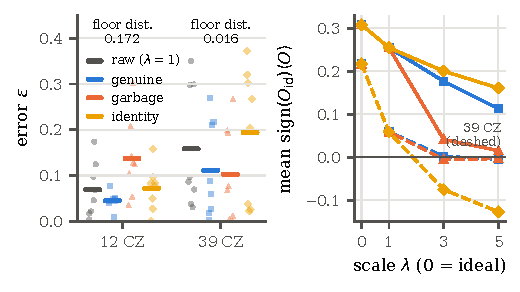
\includegraphics[width=\columnwidth]{figs/fig_zne_window.pdf}
\caption{ZNE in night A. Left: per-point errors (dots) and means (bars) of raw ($\lambda=1$),
genuine, garbage and identity folding; annotation: median floor-tracking distance of genuine
ZNE. Right: mean of $\mathrm{sign}(\Oid)\ev{O}(\lambda)$ over points, with the ideal at $\lambda=0$
(solid 12~CZ, dashed 39~CZ). At 39~CZ genuine and garbage folding coincide at the floor for
$\lambda\ge3$; identity folding drifts away from both.}
\label{fig:zne}
\end{figure}

\emph{Identity folding is not a valid control on hardware.} The identity variant has the same CZ
and PRX counts as genuine folding at every scale (checked on the archived circuits) and returns
the ideal value in noiseless simulation. On ODRA, however, its mean $\ev{O}$ drifts towards $+1$:
0.16 and 0.28 at $\lambda=3,5$ for 12~CZ, and 0.40 and 0.57 for 39~CZ, while genuine folding stays
near the floor. The cause is structural: half of each identity block is a CZ sequence without
interleaved single-qubit gates and the other half consists of gate--inverse pairs. Diagonal
gates do not mix populations, so phase errors are invisible to a $Z$ measurement, while $T_1$
relaxation towards $\ket0$ ($Z=+1$) acts unopposed. The block costs the same gates but has a
different noise from $U^\dagger U$. We draw no conclusions from it.

\emph{Cost.} ZNE uses 24,576 shots per point, CDR 1,032,192, about 42 times more. ZNE and CDR are
therefore \emph{not} compared at equal budget; Table~\ref{tab:main} reports the cost next to the
error rather than equalizing it. With this caveat, every CDR arm had a lower error than raw estimation
and ZNE at both rungs. Among the \arm{near\_target} arms, \arm{twirl\_native} was lowest at 39~CZ,
while \arm{spread} was lowest at 12~CZ (0.012) but worse than \arm{twirl\_native} at 39~CZ (0.068 vs.\ 0.040; median $r^2$ 0.69 vs.\ 0.92). The
predicted advantage of \arm{spread} concerns mainly the deepest rung (H6: \TBD{H6 result}). The
EIV fit agreed with OLS to within 0.007 everywhere except \arm{spread} at 39~CZ, where it was
worse (0.098 vs.\ 0.068)---the small true spread of $x$ under single-measurement noise is exactly
where de-attenuation is unstable.

\subsection{What drives the degradation (P5)}
Table~\ref{tab:p5} and Fig.~\ref{fig:p5} give the identity-insertion results. At fixed gate
counts, each additional microsecond raises the raw error by a factor 1.43 (95\% CI 1.30--1.58,
$p<10^{-4}$); H7b is confirmed and survives any Holm threshold (one-sided $p\approx3\times10^{-13}$).
At fixed duration, adding CZ does not raise the log raw error on average (factor 0.96 per
10~CZ, CI 0.77--1.19, $p=0.68$ two-sided; one-sided in the registered direction $p=0.66$), so
H7a is not confirmed. Point by point the picture is less stark: at each insertion level the
CZ-pair circuit has a higher raw error than its duration-matched idle twin at 6 of 8 points
(ratios 1.02--2.1), but one or two points with an accidentally near-zero error per level
(ratios down to 0.03) dominate the log-scale regression. The fair summary is that at fixed
duration the CZ effect on raw error is small and ambiguous, whereas the duration effect is
large and unambiguous.

After CDR the picture reverses: the residual error grows with CZ count (factor 1.34 per 10~CZ,
CI 1.11--1.61, $p=0.002$) and no longer significantly with duration (1.32, CI 0.77--2.27,
$p=0.31$). Including the $L=6,9,13$ classifiers, 10 additional PRX change the raw error by
1.12 (CI 0.81--1.56, $p=0.50$). The deeper classifiers fare worse than CZ insertions of the same
CZ count and similar duration, e.g.\ after CDR at 36~CZ, $L=9$ 0.135 vs.\ cz\_pairs 0.072.

\emph{Sensitivity.} Dropping the \texttt{star\_cz52} rung, in which the calibration changed, gives
raw error $\times1.48$ per \textmu s ($p<10^{-4}$) and $\times1.03$ per 10~CZ ($p=0.89$), and after
CDR $\times1.59$ per 10~CZ ($p<10^{-4}$). The pre-registered rule also flags \texttt{star\_cz24},
which ran entirely on the new calibration; dropping both rungs gives $\times1.48$ per \textmu s
($p<10^{-5}$), $\times1.03$ per 10~CZ ($p=0.87$) and $\times1.70$ per 10~CZ after CDR
($p<10^{-8}$). The conclusions are unchanged.

\begin{table}[t]
\caption{P5 regression ($L=3$ rungs, 56 observations, 8 points, point fixed effects,
SE clustered by point; $^\ast$ includes $L$=6/9/13, 80 obs.).}
\label{tab:p5}
\centering\footnotesize
\begin{tabular}{@{}llccc@{}}
\toprule
outcome & term & factor & 95\% CI & $p$ \\
\midrule
raw & +10 CZ (fixed duration) & 0.96 & 0.77--1.19 & 0.68 \\
raw & +1\,\textmu s (fixed gates) & 1.43 & 1.30--1.58 & $<10^{-4}$ \\
raw$^\ast$ & +10 PRX & 1.12 & 0.81--1.56 & 0.50 \\
after CDR & +10 CZ & 1.34 & 1.11--1.61 & 0.002 \\
after CDR & +1\,\textmu s & 1.32 & 0.77--2.27 & 0.31 \\
\bottomrule
\end{tabular}
\end{table}

\begin{figure*}[t]
\centering
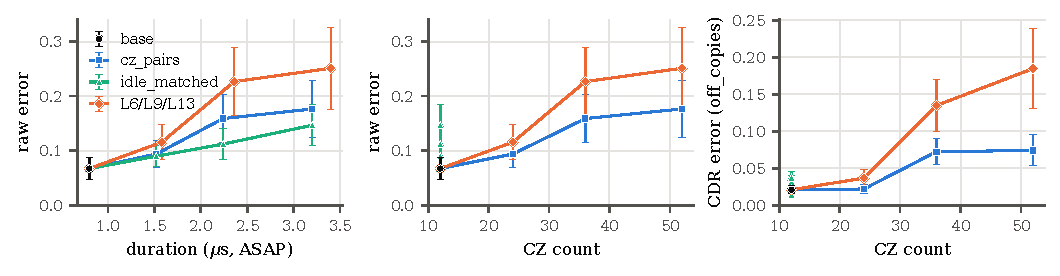
\includegraphics[width=\textwidth]{figs/fig_p5_depth.pdf}
\caption{Identity insertion (night P5, \arm{off\_copies}, OLS; mean $\pm$ SE over 8 points).
Left: raw error vs.\ ASAP duration; centre: raw error vs.\ CZ count; right: CDR error vs.\ CZ
count. Idle insertion (12~CZ) raises the raw error along the duration axis about as much as
CZ pairs do, but CDR removes most of it; the residual after CDR grows with CZ count.}
\label{fig:p5}
\end{figure*}

\subsection{The variance constant $\kappa$ (pilot, exploratory)}
$\kappa$ was not measured in \texttt{w01}. In pilot windows on the 12-CZ star circuit, it was estimated
as the intercept of $(\mathrm{MSE}_{\text{ZNE}}-\mathrm{MSE}_{\text{raw}})\cdot S$ regressed on
$S$ (budgets 256--4096, 10 repetitions), divided by $V$. For Neyman allocation the prediction
uses the measured $\sigma_k$, hence 3.06 and 11.6 rather than 3.0 and 11.25.
Table~\ref{tab:kappa} lists the results. For $\{1,3,5\}$ theory and measurement agree within
one standard error for both allocations in the first windows, and Neyman allocation lowers
$\kappa$ by about 20\%, which moves the help--harm budget $S^\ast$ down by the same factor; a
repeat of the Neyman $\{1,3,5\}$ measurement in a third window had too large an uncertainty to
be informative. $\{1,3\}$ is too noisy for a conclusion. For $\{1,3,5,7\}$ the measured
values lie well below the prediction of $\approx37$ in both windows; possible reasons are the
variance model at $\lambda=7$, correlations between scales within a window, or a non-linear
dependence of the MSE difference on $S$. This remains open.

\begin{table}[t]
\caption{Pilot measurement of $\kappa$ (ODRA, 12-CZ star; exploratory).}
\label{tab:kappa}
\centering\footnotesize
\begin{tabular}{@{}llcc@{}}
\toprule
nodes & allocation & measured & predicted \\
\midrule
$\{1,3,5\}$ & uniform & $15.8\pm1.7$ & 14.66 \\
$\{1,3,5\}$ & Neyman & $12.5\pm1.1$; $20.7\pm14.7$ & 11.6; 11.9 \\
$\{1,3\}$ & Neyman & $1.3\pm1.3$ & 3.06 \\
$\{1,3,5,7\}$ & Neyman & $26.0\pm3.3$; $25.7\pm11.3$ & 36.7; 37.2 \\
\bottomrule
\end{tabular}
\end{table}

\subsection{Classifier decisions}
A decision changes from $E$ to $\hat O$ only if $|\hat O-E|\ge|E|$; bounded corrections can
therefore flip only small-$|E|$, i.e.\ small-margin, points. In night A (16 points), the
raw target of the \arm{twirl\_native} arm agreed with the ideal decision at 15/16 points and
the mitigated value at 16/16; the single change (a repair) occurred at a point of margin
0.028, while the median margins of the two rungs were 0.31 and 0.16. ZNE agreed at 16/16
points. \TBD{H5 McNemar on 32 pairs and changes below the median margin}.

\emph{Pilot (exploratory).} A pilot with 100 reference points per rung (ladder 12/30/39/57,
$n_{\text{train}}=100$, one CDR fit per rung, 8192 shots) gives Table~\ref{tab:dec}. All 31
decision changes under CDR and all 18 under ZNE fall in the half of the points with margin
below the median; under independence of margin this would have probability of order
$2^{-31}$. Better $\ev{O}$ estimates need not change decisions, and when they do, it is near
the boundary.

\begin{table}[t]
\caption{Pilot decision agreement with the ideal classifier (100 points per rung); $b$:
raw correct, mitigated wrong; $c$: the reverse; exact McNemar $p$, uncorrected.}
\label{tab:dec}
\centering\footnotesize
\begin{tabular}{@{}rccccc@{}}
\toprule
CZ & raw$\to$CDR & $b/c$ & $p$ & raw$\to$ZNE & $b/c$ \\
\midrule
12 & 0.99$\to$0.96 & 4/1 & 0.38 & 0.99$\to$0.96 & 3/0 \\
30 & 0.87$\to$0.92 & 0/5 & 0.06 & 0.87$\to$0.92 & 0/5 \\
39 & 0.83$\to$0.93 & 0/10 & 0.002 & 0.83$\to$0.89 & 0/6 \\
57 & 0.90$\to$0.97 & 2/9 & 0.07 & 0.90$\to$0.92 & 1/3 \\
\bottomrule
\end{tabular}
\end{table}

% ---------------------------------------------------------------------------------------
\section{Discussion}\label{sec:discussion}

\emph{A regime map.} Along the ladder measured so far, the picture is: raw estimation for the
smallest budgets; ZNE as the cheap option, genuine at 12~CZ but an artefact from 39~CZ on; CDR
(with twirling where a systematic error remains) as the lowest-error option from 12~CZ on, at roughly 42 times the shots of ZNE.
Twirling pays where there is a systematic error left for it to remove (39~CZ) and not where CDR
is already at its statistical floor (12~CZ). Two axes from Section~\ref{sec:background} organize
the map: along the budget axis the ZNE threshold $S^\ast=\kappa V/(B^2-B^2_{\text{ZNE}})$, whose
node-only constant $\kappa$ the pilot supports for $\{1,3,5\}$; along the depth axis the signal
collapse that closes the ZNE window. Where on the ladder between 12 and 39~CZ the ZNE window
closes, and whether twirled CDR keeps its lead at 57~CZ, is \TBD{night-B regime boundary}.

\emph{Why CDR absorbs time-driven decay but not CZ-driven error.} Relaxation and dephasing during
the schedule act, to a first approximation, as a contraction of the signal that is common to all
circuits with the same schedule---the training circuits share the target's skeleton, insertions
and timing. That is the affine map CDR is built to learn, which explains why idle insertion
barely affects the CDR error (Fig.~\ref{fig:p5}, right) although it raises the raw error as much
as CZ pairs do. The CZ-driven part is different: whatever its microscopic form, its effect on
$\ev{\bar Z}$ depends on the specific single-qubit content of the circuit, so a line learned on
Clifford versions transfers worse, and $r^2$ drops (e.g.\ at 36 and 52~CZ in P5, median $r^2$
0.81 and 0.67 against 0.94 and 0.87 for the idle twins). This is consistent with twirling, which
acts on the CZ noise, helping CDR at the deeper rung. We do not claim that the twirling gain is
explained by a coherent $ZZ$ error on the CZ: twirling helps empirically, but the mechanism goes
beyond a simple coherent $ZZ$ error on the CZ, and identifying it is left to device-calibrated
modelling.

\emph{A lesson from the failed control.} Identity folding was designed as the positive
counterpart of garbage folding and passed every structural and simulated check, yet on hardware
it measured something else. A control that matches gate counts does not necessarily match
noise. Matched-cost controls must be validated on the device, not only in simulation, and a
control whose function is destroyed (garbage) is more robust than one whose function is preserved
by a different gate arrangement (identity). Conversely, $W_{\text{neg}}$ and SNR, both
plausible collapse diagnostics, passed a rung that the garbage control exposed; we recommend
that hardware ZNE results be reported with a garbage-folding control.

\emph{Limitations.} (i) \textbf{One device.} All new data come from ODRA~5 and its star topology;
on lattices (IQM Garnet, Emerald) the same function costs a different number of CZ and the noise
has a different structure, so the boundaries will move. (ii) \textbf{Few points.} Each rung has 8
evaluation points; per-rung tests are weak, and the 12-CZ geometric ratio shows how two
near-zero errors can dominate a log-scale summary. (iii) \textbf{One calibration window.} Stability
of the effects across calibrations (pre-registered as untestable within w01) is not addressed,
and one P5 block changed calibration mid-run. (iv) \textbf{Pre-analysis, not pre-data,
registration}, as stated in Section~\ref{sec:methods}. (v) \textbf{ZNE and CDR are not budget-matched}
(24,576 vs.\ 1,032,192 shots per point); equal budgets hold only among CDR arms. (vi) \textbf{The
identity-folding control is invalid on hardware} and was excluded. (vii) \textbf{One workload}:
a mean-$Z$ observable on a five-qubit classifier, whose Clifford ideal values are often zero at
depth; other observables change both the floor and the training-set informativeness. (viii) The
$\kappa$ and decision results are pilot data on earlier runners; the pilot CDR used a single fit
per rung. (ix) Night B (30 and 57~CZ) is \TBD{pending}, so the pre-registered confirmatory
tests H1, H3 and H6 are not yet reported.

% ---------------------------------------------------------------------------------------
\section{Conclusion}
On a five-qubit star processor, with mitigation arms compared at equal shot budgets and ZNE
accompanied by matched-cost controls, we find that (1) Pauli twirling lowers the CDR error by
about 30\% at 39~CZ and does nothing at 12~CZ, where CDR is already at its statistical floor;
(2) ZNE is genuine at 12~CZ but at 39~CZ its gain over raw estimation is an artefact of signal
collapse that only the garbage-folding control detected; (3) raw error is driven by circuit
duration rather than CZ count at fixed duration, while the error that survives CDR is the
CZ-driven part. The same protocol is designed to transfer to lattice devices, where the routing
ladder and the noise structure differ. \TBD{one-sentence conclusion from night B}.

\section*{Data and code availability}
Raw counts (\texttt{counts.jsonl}), manifests, derived tables, the frozen models, the
pre-registration (tag \texttt{prereg-v1}) and the analysis and figure scripts will be made
available at \TBD{repository URL / DOI}.

\section*{Acknowledgment}
\TBD{acknowledgments: access to ODRA~5, KN Axion, funding}.

\bibliographystyle{IEEEtran}
\bibliography{refs}

\end{document}
